\documentclass[letterpaper,11pt]{report} %tipo de documento y tamaño de papel y letra
\usepackage[latin1]{inputenc} %codificación de caracteres
\usepackage[spanish]{babel} %idioma
\usepackage{fancyhdr} %tipo de página, LINDA biggrin.gif
\usepackage[top=3.5cm,bottom=2.5cm,right=2cm,left=2.5cm]{geometry} %márgenes
\usepackage[rflt]{floatflt} %ni puta idea
\usepackage{pdfpages} %incluir archivos pdf
\usepackage{hyperref} %hipervinculos
\hypersetup{
  colorlinks=true,
  urlcolor=cyan
}
%\usepackage{helvet} %esto es pa escribir con Arial en vez de times new roman
%\renewcommand\familydefault{\sfdefault} %descomenta estas lineas para escribir en arial

\usepackage{multirow}

\usepackage{graphicx} %para usar imagenes
%\newcommand{\imgdir}{doc-img} % para meter las imágenes en una carpeta especial, tunz en la carpeta del documento tiene q ir otra que se llame 'doc-img'
\graphicspath{{./pic/}} %le dice que las imágenes están en la carpeta de arriba

\usepackage{amsmath} %pa usar símbolos matematicos
\numberwithin{equation}{section} % pa usar ecuaciones de modo lindo
\numberwithin{figure}{section} %para agregar imágenes
\numberwithin{table}{section} %para agregar tablas

\usepackage{subfigure} % pa usar sub figuras



\pagestyle{fancy} %configuración para la pagina linda
\renewcommand{\sectionmark}[1]{\markboth{}{\thesection\ \ #1}} %cambios de comentarios
\lhead{} %parte de arriba, izq
\chead{} %parte de arriba, centro
\rhead{\rightmark} %parte de arriba, derecha, le agrega la marca del capitulo
\lfoot{} %parte de abajo, izq
\cfoot{} %parte de abajo, centro
\rfoot{\thepage} %parte de abajo, derecha, va el numero de la página


%-------------portada---------------------------------%
\begin{document}
\begin{titlepage} %portada
\thispagestyle{empty} %borrar el formato de pagina linda
%\begin{flushleft} %alinear a la izq
\begin{center}

\includegraphics[scale=0.25]{logoUSM-DI.eps}
%\vfill
\end{center}
%\end{flushleft}

\vspace{3cm} %espacio vertical , en realidad es un enter de 2 cm
\begin{center} %centrar
{\Huge Proyecto ``\emph{V.I.Pe.R.}''\\
 \huge Pre-Empresa {\bf Phyrex} \\
  \normalsize\today
}
\end{center}

\vspace{2cm}
\begin{flushleft}
\begin{table}[h]
    \begin{tabular}{lp{13cm}}
      {\Large \bf Descripci\'on:} & {\large Simulador de mascota que explota caracter\'{\i}sticas de smartphones Android e interact\'ua con robot Lego, enfocado en la difusi\'on del Dpto. de Inform\'atica de la UTFSM.}\\
      & \\
      & \\
      {\Large \bf Problema:} & {\large En las carreras inform\'aticas se encuentre una gran desinformaci\'on respecto a si mismas, adem\'as de una disminuci\'on en la tasa de matr\'{\i}culas anuales, tanto a nivel nacional como mundial, en particular en el caso de la UTFSM.}\\
    \end{tabular}
\end{table}
\end{flushleft}

%\vspace{6cm}
\vfill
\begin{flushleft} %alinear derecha
\begin{table}[hb]
  \begin{tabular}{lllc}
    Jefe de Proyecto: & Rodrigo Fr\'{\i}as & \texttt{\small <rodrigo.frias@alumnos.usm.cl>} & [+56 9 83988257] \\
    Equipo: & Celeste Bertin & \texttt{\small <celeste.bertin@alumnos.usm.cl>} &[+56 9 68410901]\\
    & Patricio Carrasco &\texttt{\small <patricio.carrascod@alumnos.usm.cl>} &[+56 9 50626689]\\
    & Rocio Fernandez &\texttt{\small <rocio.fernandezu@alumnos.usm.cl>} &[+56 9 62426549]\\
    Categor\'{\i}a: & \multicolumn{3}{l}{Educaci\'on \& Entretenimiento.}\\
    Campus: & \multicolumn{3}{l}{Santiago San Joaqu\'{\i}n.}
  \end{tabular}
\end{table}
\end{flushleft}
\end{titlepage}
%------------------fin de la portada --------------------%

%{\bf } %escribir en negrita

\setcounter{page}{1} %empezar enumerando la página 1

\tableofcontents %índice
\newpage

\chapter*{Propuesta T\'ecnica}
\newpage
\section{Identificaci\'on del problema u oportunidad}

\newpage
\section{Visualizaci\'on de una soluci\'on}

\newpage
\section{Innovaci\'on}

\newpage
\chapter*{Anexo I - Presentaci\'on} %Copia Presentacion
\includepdf[pages={1-},frame=true,nup=2x3]{../Presentacion/diapo-1x1.pdf}
\newpage
\chapter*{Anexo II - Curr\'{\i}culum Vitae} %Curriculum
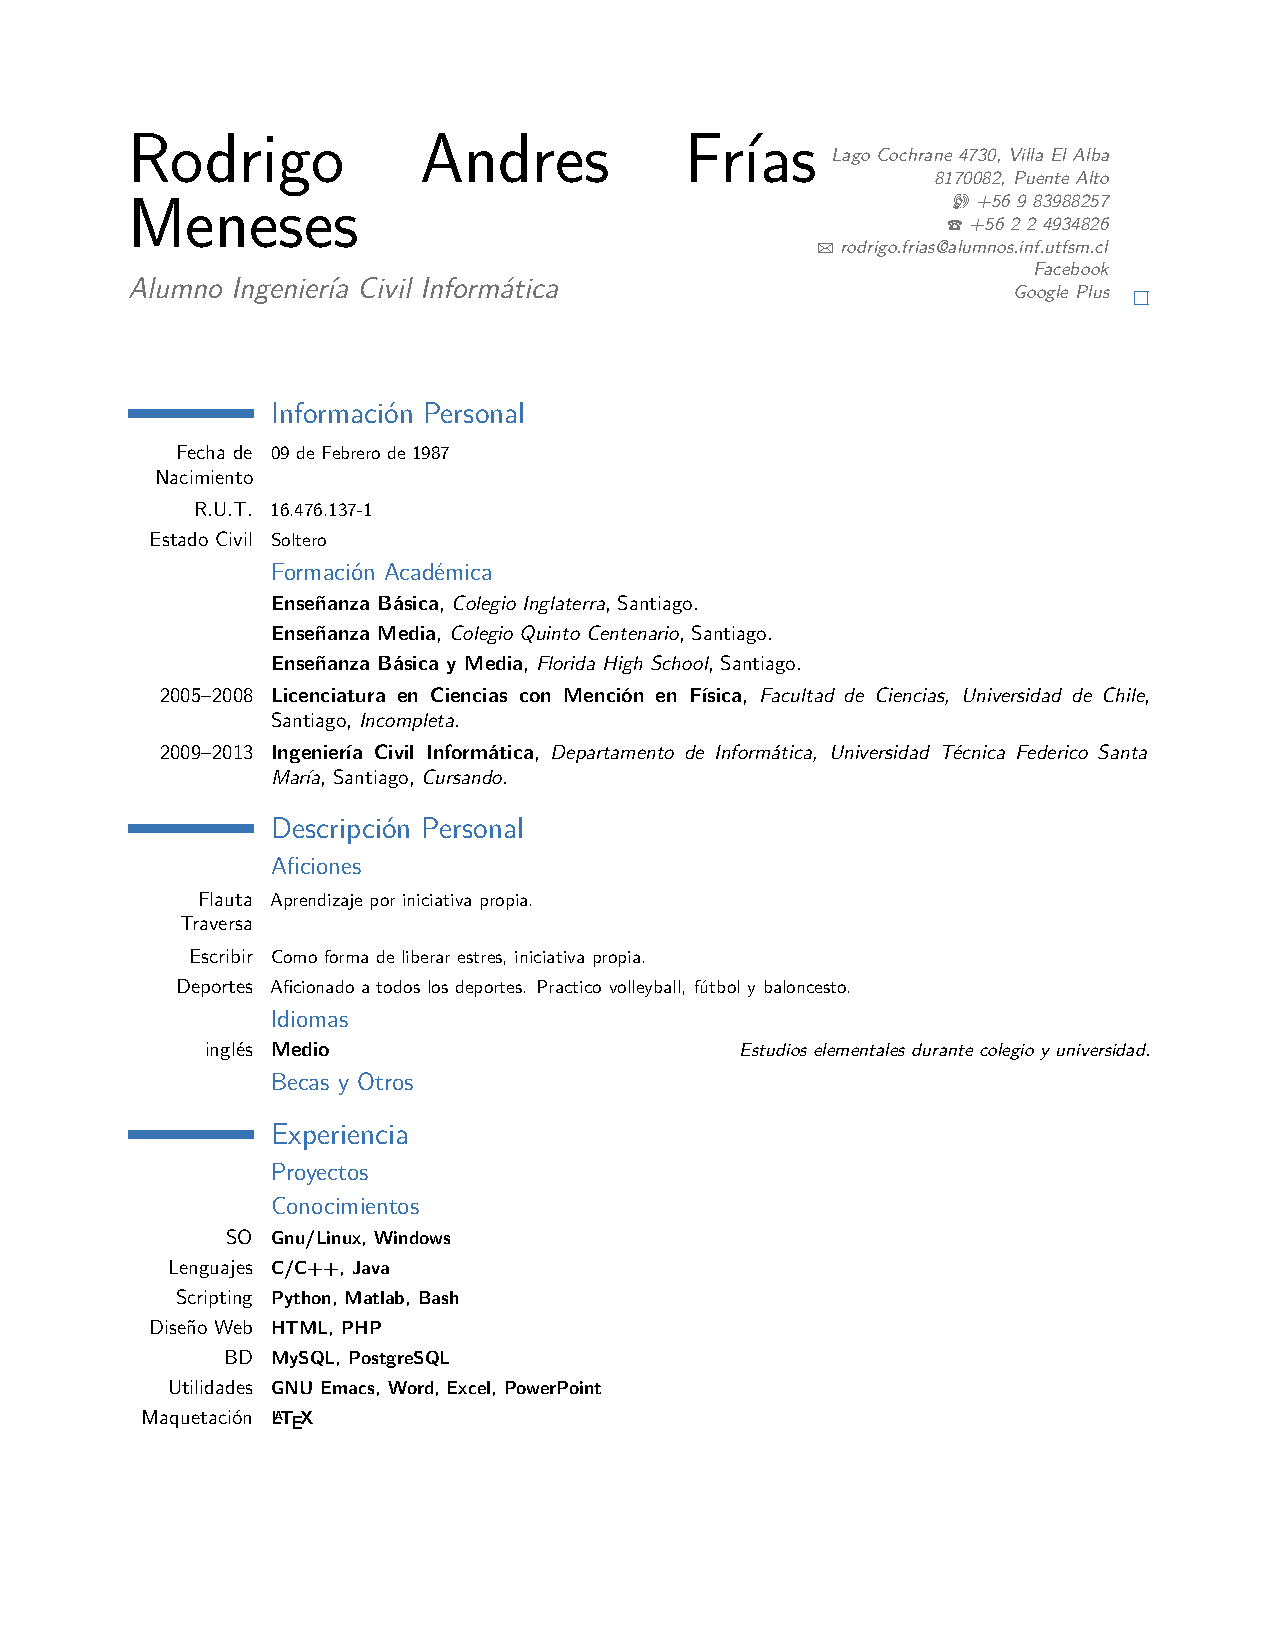
\includepdf[pages={1}]{../CV/cv-igo.pdf}
\includepdf[pages={1}]{../CV/cv-celeste.pdf}
\includepdf[pages={1}]{../CV/cv-pato.pdf}
\includepdf[pages={1}]{../CV/cv-neko.pdf}
\newpage
\chapter*{Anexo III - Otros} %Otros


\end{document}
